\documentclass[12pt]{article}
\usepackage{amsmath, amsfonts, enumerate, epsfig, cite, wrapfig}
\usepackage[leftcaption]{sidecap}
\usepackage{epstopdf}
\usepackage[margin=0.5in]{geometry}

\usepackage[super,comma,compress]{natbib}
\usepackage[skip=0pt]{caption}
\usepackage{subcaption}
\usepackage{mathtools,amssymb}
\usepackage{amsmath}
\usepackage{breqn}
\sidecaptionvpos{figure}{t}
\setlength{\belowcaptionskip}{0mm}
\setlength{\intextsep}{-2mm}
\renewcommand{\figurename}{\small Figure}
\renewcommand{\refname}{}

\DeclareMathOperator*{\argmax}{arg\,max}

\renewcommand\floatpagefraction{.9}
\renewcommand\topfraction{1}
\renewcommand\bottomfraction{1}
\renewcommand\textfraction{0}   
\setcounter{totalnumber}{50}
\setcounter{topnumber}{50}
\setcounter{bottomnumber}{50}

\newlength{\toppush}
\setlength{\toppush}{2\headheight}
\addtolength{\toppush}{\headsep}

\pagestyle{empty}
\begin{document}
\noindent{\bf Title}: Degenerate solution networks (DSNs) for theoretical neuroscience \\
\noindent{\bf Author list}: Sean R. Bittner and John P. Cunningham \\

\noindent Theoretical neuroscientists design and test mathematical models of neural activity, assessing a model's quality by its ability to replicate experimental results.  A general challenge has been addressing the indeterminacy of model parameterizations; different parameterizations of these models accurately reflect established experiments, yet make incompatible predictions about other aspects of neural activity.  We present a novel machine learning methodology called degenerate solution networks (DSNs), which learn the full (i.e. maximum entropy) distribution of generative model parameterizations that yield a behavior of interest.  DSNs are a tool designed for theorists, that enables a new class of model analyses relying on the full distribution of generative parameters that result in some statistically specified activity. For example, consider the stomatogastric ganglion (STG) circuit in the crustacean, which generates tri-phasic rhythms and has a well-studied biophysical model.  Rather than examining the parameter space of this model though extensive simulation \cite{prinz2004similar} as is common practice, we could directly learn the maximally random distribution of channel conductances and synaptic efficacies that yield tri-phasic rhythms with a DSN.  Here, we demonstrated the utility of DSNs in three (of many possible) use cases.  First, we learned the degenerate solution space of 2D linear systems producing a band of pure oscillations.  Then, relying on input-driven dynamic mean field theory \cite{mastrogiuseppe2018linking}, we use DSNs to study solution spaces of recurrent neural networks (RNNs), one of the most widely used models in theoretical neuroscience.  Finally, in contrast to RNNs, we discuss using DSNs to learn the parametric solution space of biophysically realistic models such as the STG.  More generally, we speculate that access to such degenerate parameterizations can facilitate model comparison, inform model revision, and guide experimental design.  \\

\vspace{-4pt}
\noindent\makebox[\linewidth]{\rule{\columnwidth}{0.4pt}}
\setlength{\abovecaptionskip}{-3mm}
\begin{wrapfigure}{b}{.45\textwidth}
  \begin{center}  
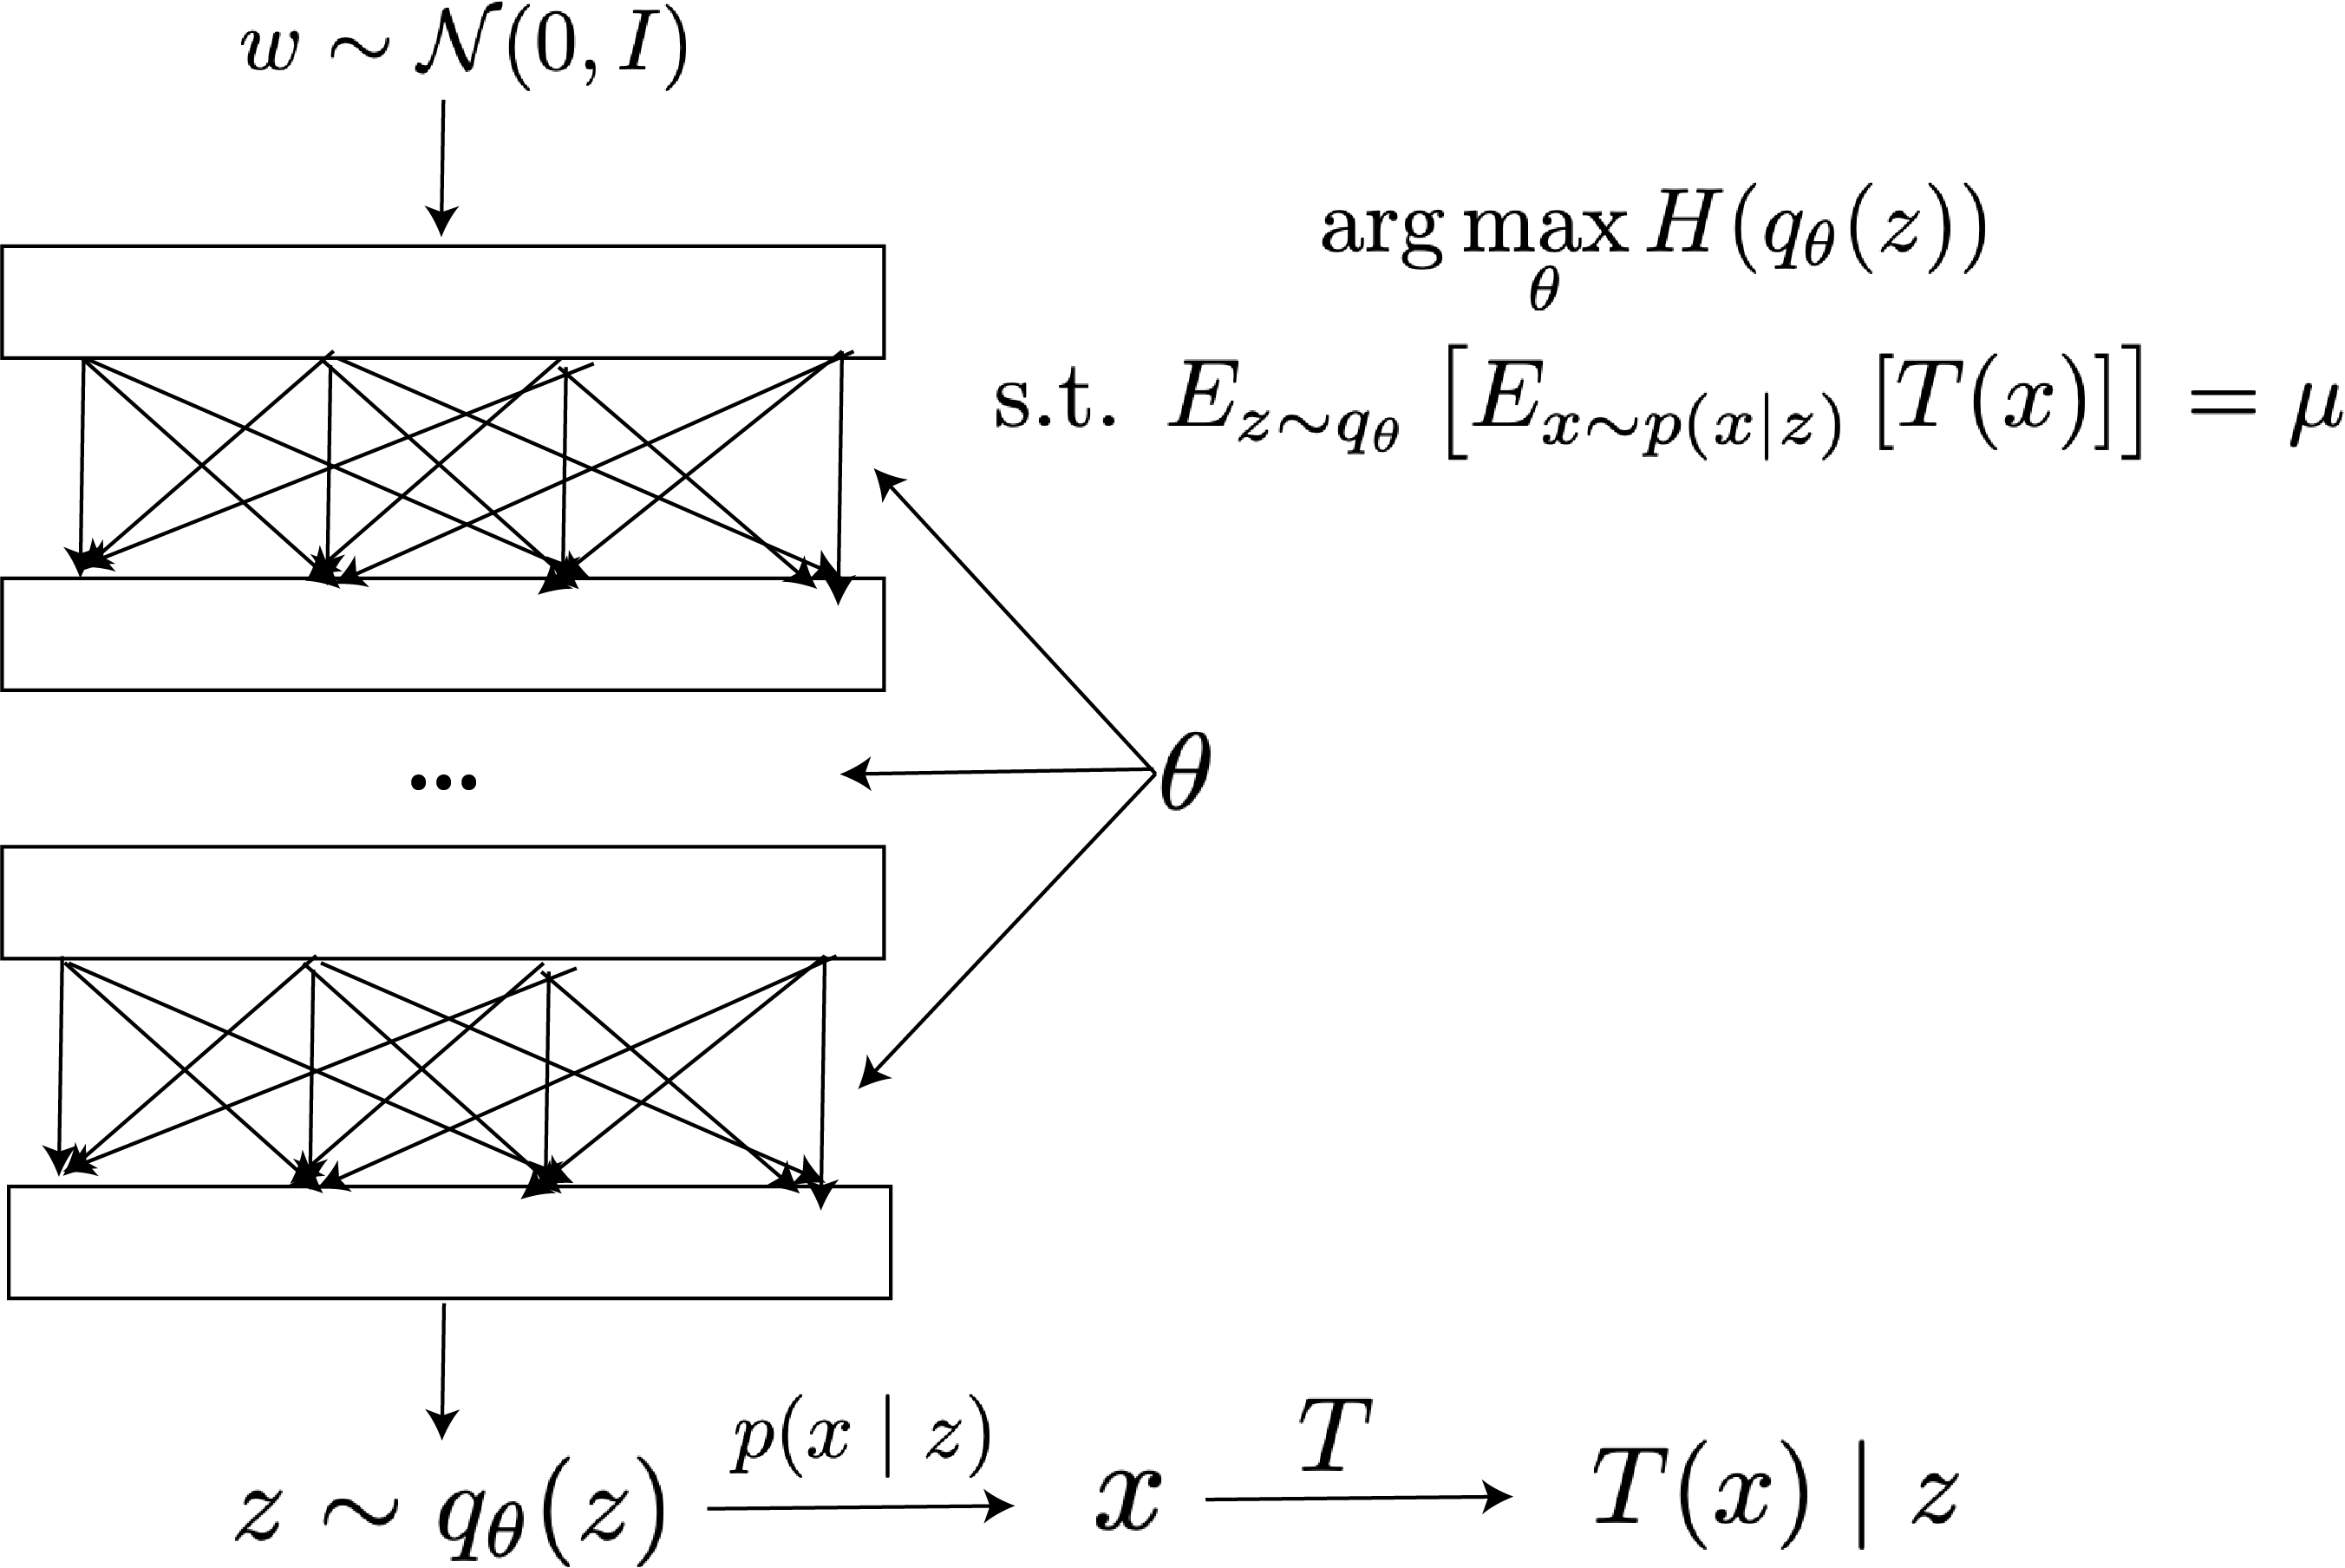
\includegraphics[scale=.3]{images/CosyneAbstract/DSN.png} 
\end{center}
 \caption{\label{fig:fig1} Degenerate solution network}\end{wrapfigure}
 
\noindent \textbf{Methods}:
\noindent Consider model parameterization $z$ and data $x$ generated from some generative model of interest with known sampling procedure and likelihood $p(x \mid z)$, which may or may not be known.  Returning to the STG example, we have a known sampling procedure for simulating activity given a circuit parameterization, yet lack an explicit likelihood function for the generated neural activity due to the complex nonlinear dynamics. DSNs learn a distribution on parameters $z$, that yields a behavior of interest $\mathcal{B}_i: E_{z \sim q_\theta}\left[ E_{x\sim p(x \mid z)}\left[T_i(x)\right] \right] = \mu_i$ by making a deep generative model approximation \cite{rezende2015variational} $q_\theta(z)$ to $p(z \mid \mathcal{B})$.  In deep generative models, a simple random variable $w \sim p_0$ is mapped deterministically via a function $f_\theta$ parameterized by a neural network to the support of the distribution of interest where $z = f_{\theta}(w)$.  DSNs are trained by optimizing the deep generative parameters $\theta$ to find the optimal approximation $q_{\theta}^*$ within the deep generative variational family $Q$ to $p(z \mid \mathcal{B})$. This procedure is loosely equivalent to variational inference (VI) using a deep generative variational family with respect to the likelihood of the mean sufficient statistics rather than the data itself \cite{loaiza2017maximum, bittner2018learning}.  In most settings (especially those relevant to theoretical neuroscience) the likelihood of the behavior with respect to the model parameters $p(T(x) \mid z)$ is unknown or intractable, requiring an alternative to stochastic gradient variational bayes \cite{kingma2013auto} or black box variational inference \cite{ranganath2014black}. Instead, DSNs are optimized with the following objective for a given generative model and some statistical constraints on its produced activity:
\begin{equation}
\begin{split}
q_\theta^*(z) &= \argmax_{q_\theta \in Q} H(q_\theta(z)) \\
 &  \text{s.t.  } E_{z \sim q_\theta}\left[ E_{x\sim p(x \mid z)}\left[T(x)\right] \right] = \mu \\
 \end{split}
\end{equation}

 \setlength{\abovecaptionskip}{-3mm}
\begin{wrapfigure}{b}{.45\textwidth}
 \caption{\label{fig:fig2} Pairplot of oscillating 2D linear system degenerate solution distribution }
  \begin{center}  
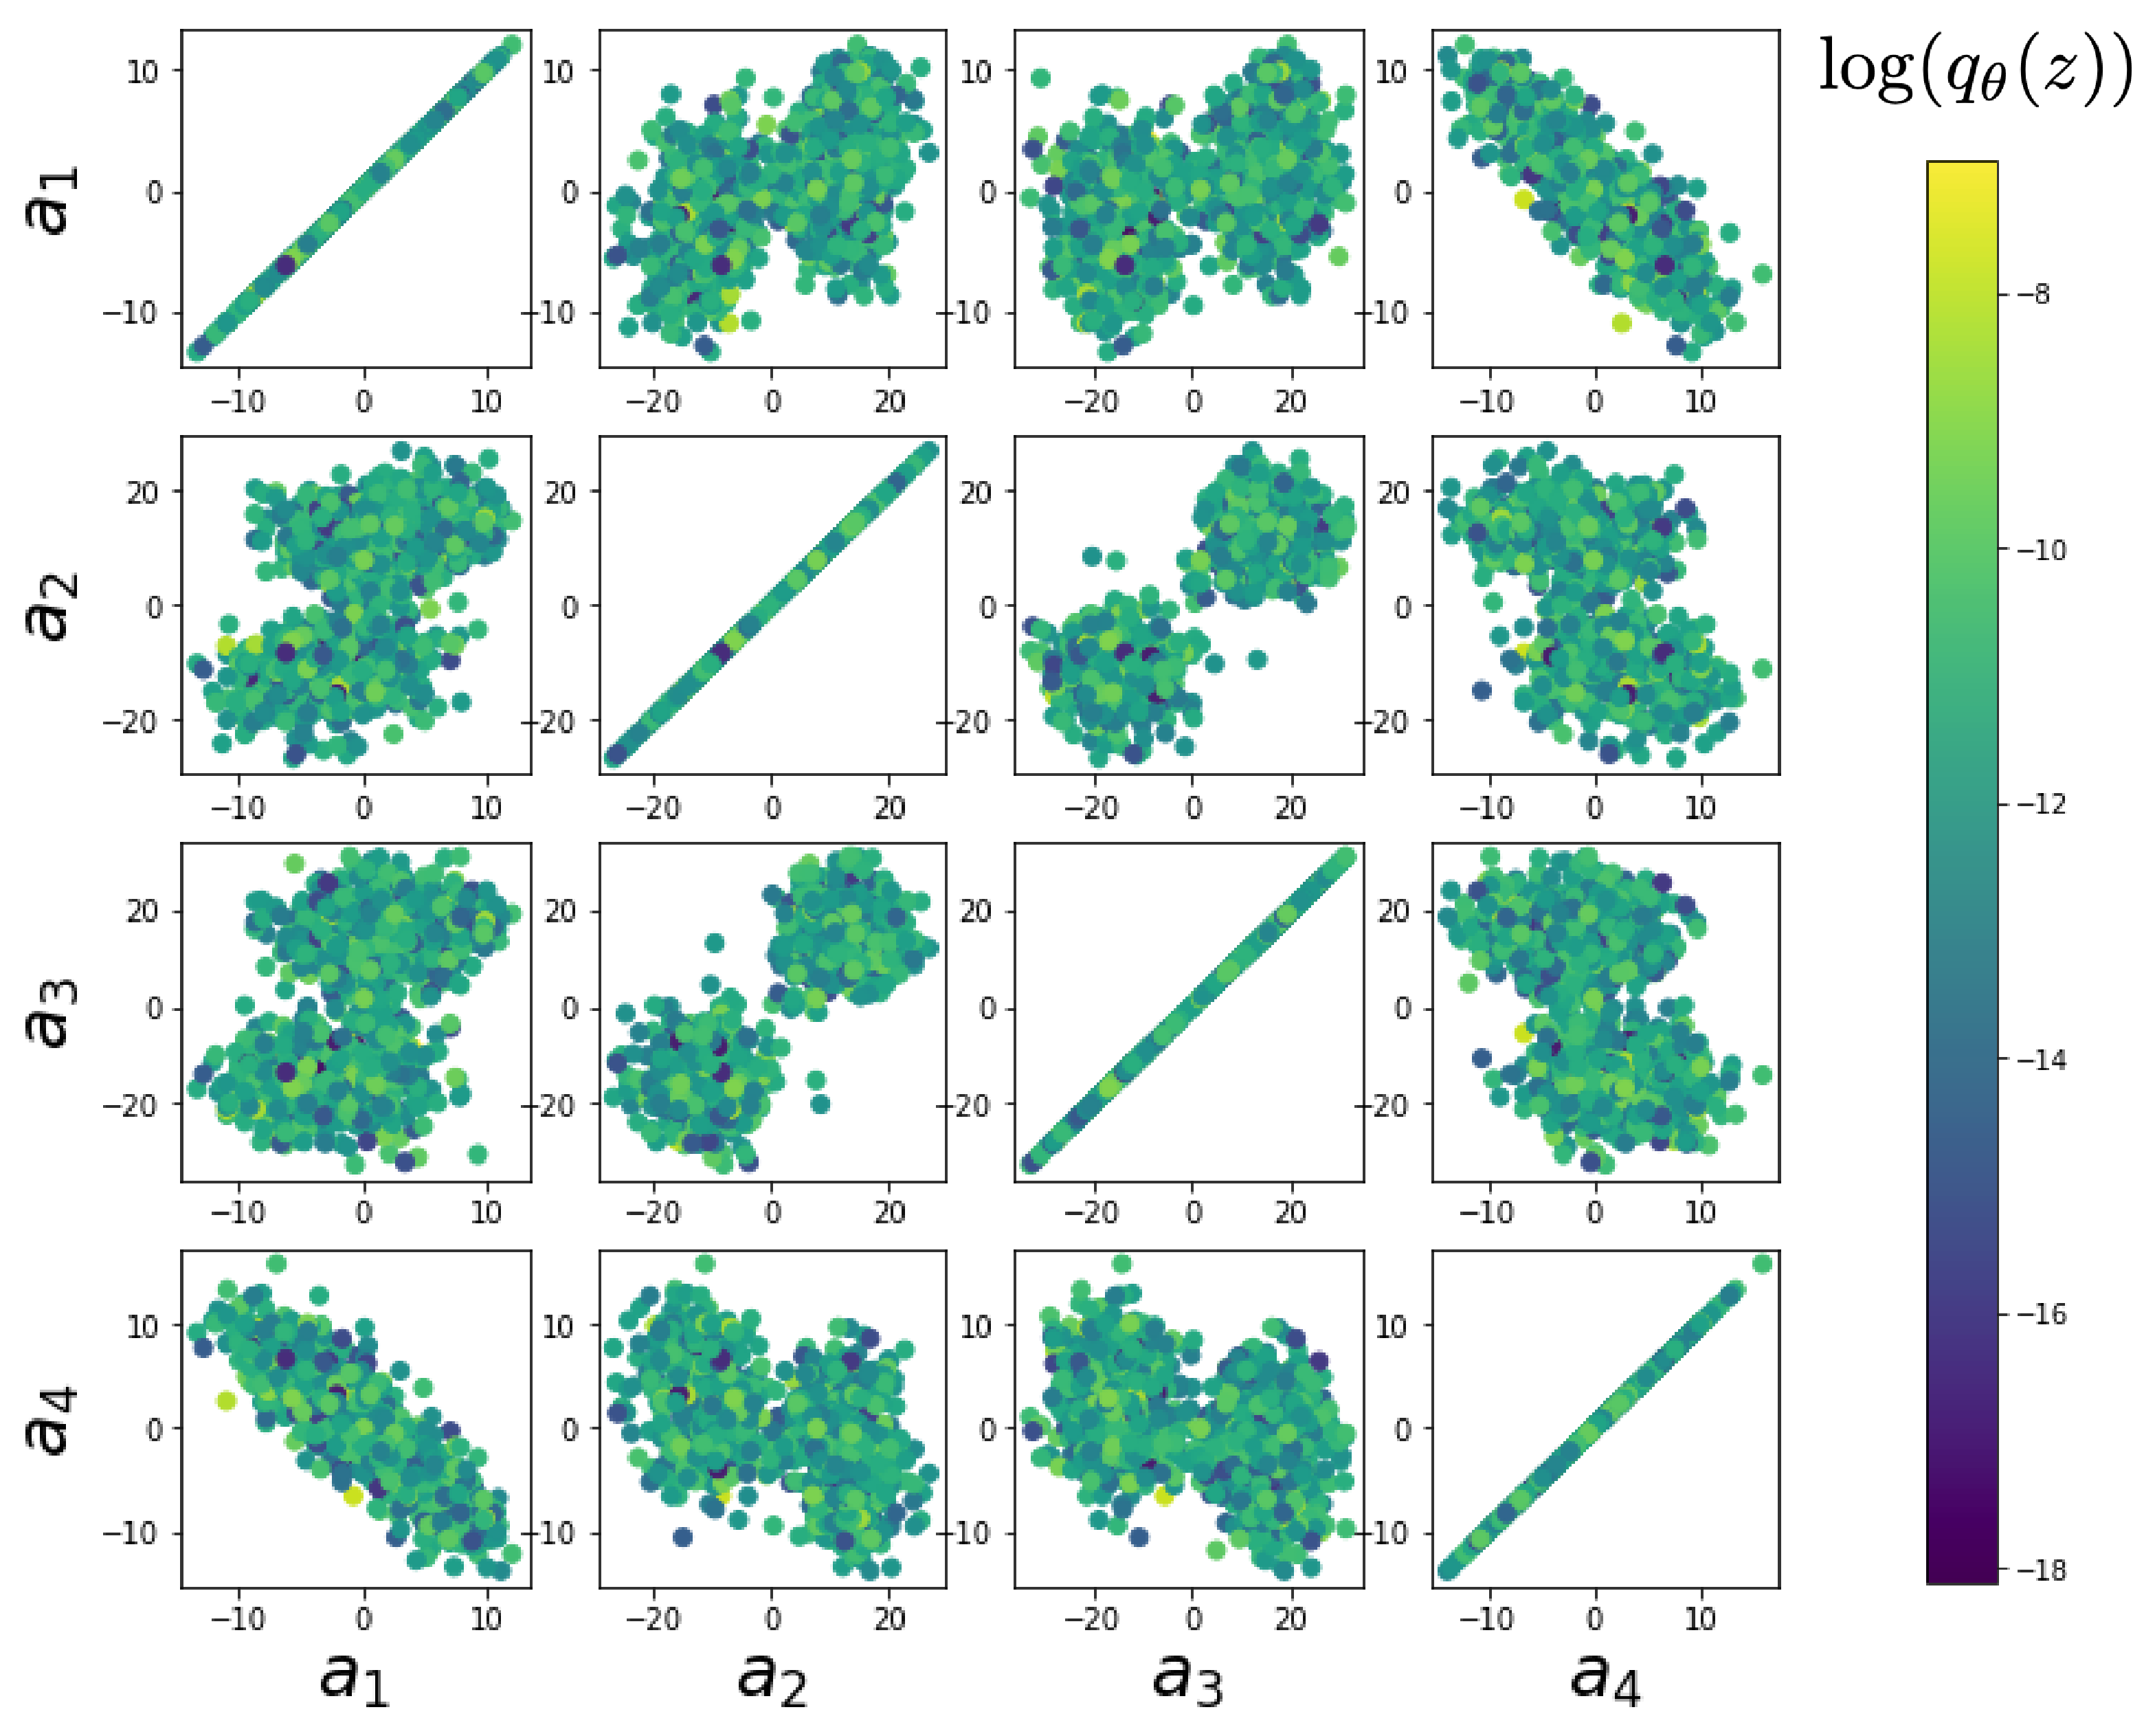
\includegraphics[scale=.3]{images/CosyneAbstract/Fig2.png} 
\end{center}
\end{wrapfigure}

\paragraph{Results: Linear Systems}   To provide intuition for DSNs to the reader, we discuss degenerate parameterizations of two-dimensional linear dynamical systems, $\dot{x} = Ax$ with $A = \begin{bmatrix} a_1 & a_2 \\ a_3 & a_4 \end{bmatrix}$ that produce a band of oscillations. To train a DSN to learn the maximally entropic distribution of real entries of the dynamics matrix $z = \left[a_1, a_2, a_3, a_4 \right]$ that yield a band of oscillations, we choose $T(x)$ to contain the first- and second-moments of the oscillatory frequency and the real part of the eigenvalues of the oscillating system, with $\mu = E \left[\text{real}(\lambda), \text{real}(\lambda)^2, \text{imag}(\lambda), \text{imag}(\lambda)^2\right] = \left[0.0, 1.0, 4\pi, 1.0 \right]$. Even though we can compute $E_{z \sim q_\theta}\left[ E_{x\sim p(x \mid z)}\left[T(x)\right] \right]$ via the eigenvalues of $A$, we cannot derive the distribution $q^*_\theta$, since the backward mapping from the mean parameters $\mu$ to the natural parameters $\eta$ of this exponential family is unknown.  Instead, we can train a DSN to learn the degenerate linear system parameterization (Fig. 2). Even this relatively simple system has nontrivial (though intuitively sensible) structure in the parameter distribution.  Indeed, more subtle model-behavior combinations will have even more complexity, further motivating DSNs. \\

\noindent \textbf{Results: Richer DSN models}: RNNs are often trained to execute computations in order to perform some experimental task with the intention of comparing the trained system's activity with that measured in the brain.  There are a variety of methods used to train RNNs, and how these learning methods bias the learned connectivities (and potentially the implemented algorithm) within the broader solution space remains poorly understood.  An assessment of the degenerate parameterizations of RNNs that solve a given task would be valuable for characterizing learning algorithm biases, as well as other analyses.   Recent work on low-rank RNNs \cite{mastrogiuseppe2018linking} provides statistical descriptions of RNN behavior.  We use this theory to compute $T(x)$ when training DSNs to learn maximum entropy distributions of network connectivities that solve a task.  More specifically, rank-1 RNNs with $N$-neurons have connectivity $J = gX + P$, which is parameterized by two $N$-length vectors $m$ and $n$ such that $P$ = $\frac{mn^\top}{N}$ and a disorder term $g$, that scales the random component $\mathcal{X}$, where $\mathcal{X}_{ij} \sim \mathcal{N}(0, \frac{1}{N})$.  Input-driven dynamic mean field theory (DMFT) requires gaussian parameterizations of the elements of $m$ and $n$, where $m_i \sim \mathcal{N}(M_m, \Sigma_m^2)$ and $n_i \sim \mathcal{N}(M_n, \Sigma_n^2)$.  We train DSNs to learn distributions of $z = \left[M_m, M_n, \Sigma_m, \Sigma_n, g\right]$ that solve the Go No-Go task, in which networks respond in the readout dimension to stimulus A, but have no response to stimulus B.

\noindent In contrast to abstract computational models, we consider using DSNs to learn the solution space of a biophysical model of the STG.  This  conductance-based neural circuit model is comprised of three neurons (AB/PD, LP, and PY) with seven synapses connecting them.  The model parameters are the synaptic efficacies and the channel conductances of each neuron.  We are interested in learning the full distribution of circuit parameterizations that yield tri-phasic rhythms, in which the three neurons burst in  a regular sequence: AB/PD, LP, then PY.  Satisfactory tri-phasic rhythms can be specified by a gaussian distribution on generated neural activity characteristics such as bursting onset lags, burst rates, and duty cycles.  As before, these metrics of activity and their targets form the $T(x)$ and $\mu$ of the DSN.  However, this circuit behavior $T(x)$ has no closed form description with respect to the parameters, as with linear systems, or with the low-rank RNNs using DMFT.  Therefore we need to simulate this biophysical circuit, and directly measure $T(x)$ on each iteration of optimization in the DSN learning algorithm.  This can be quite expensive, so we are actively researching ways to make DSNs scale to such complex behavioral characterizations.

\noindent



\noindent [1] A Prinz et al., 2004. [2] Mastrogiuseppe \& Ostojic, 2018. [3] Rezende \& Mohamed, 2015. [4] Loaiza-Ganem et al., 2017. [5] Bittner \& Cunningham. (In review), 2018.  [6] Kingma \& Welling, 2013.

 \noindent [7] Ranganath et al., 2014.

\bibliography{dsn}
\bibliographystyle{unsrt}

\end{document}

